\documentclass{book}

% 本文必要宏包
\usepackage{amssymb}
\usepackage{amsmath}
% \usepackage{graphicx}
% \usepackage{multirow}
% \usepackage{paralist}
% \usepackage{color}
% \usepackage{float}
\usepackage{nicematrix}
% \usepackage{tikz}
% \usetikzlibrary{matrix,decorations.pathreplacing}
\usepackage{arydshln} %虚线
\usepackage{algorithm} % 算法
\usepackage{algmatlab} % matlab风格代码

% 参考文献管理
% \usepackage{titlesec}
% \titleformat{\chapter}[display]{\normalfont\huge\bfseries}{}{0pt}{}
% \titlespacing*{\chapter}{0pt}{-40pt}{0pt}
% \renewcommand{\bibname}{}
% \usepackage[numbers,sort&compress]{natbib}

% % elsarticle依赖包
% \usepackage{natbib} % 引文处理
% \usepackage{geometry} % 页边距设置
% % \usepackage{fleqn} % 左对齐公式
% \usepackage{graphicx} % 插入图形


% % 其他数学环境
% \newtheorem{theorem}{Theorem}[section]
% \newtheorem{definition}[theorem]{Definition}
% \newtheorem{lemma}[theorem]{Lemma}
% \newtheorem{corollary}[theorem]{Corollary}
% \newtheorem{proposition}[theorem]{Proposition}
% \newtheorem{example}[theorem]{Example}
% \newtheorem{remark}[theorem]{Remark}
% \newenvironment{proof}{\noindent {\bf Proof.\ }}{\vspace{2ex}}

% \numberwithin{equation}{section}

% \biboptions{numbers,sort&compress}

% \usepackage[style=authoryear]{biblatex}
% \addbibresource{references.bib}
\usepackage{cite}
%%%%%% 引用链接,方便引用跳转可以去掉
\usepackage{hyperref}
\hypersetup{colorlinks=true, citecolor=blue}
%%%%%% 

%%%%% 以下为杂志特定
\usepackage{latexsym}
\usepackage{bm}
%%%%%%%%%%%%%%%%%%%%force formula number size unchanged
\makeatletter
\def\my@tag@font{\normalsize}
\def\maketag@@@#1{\hbox{\m@th\normalfont\my@tag@font#1}}
\let\amsmath@eqref\eqref
\renewcommand\eqref[1]{{\let\my@tag@font\relax\amsmath@eqref{#1}}}
\makeatother
\usepackage{amssymb}
\usepackage{color}
%%%%%%%%%%%%%%%%%%%%%%%%%%set table background color
\usepackage{colortbl}
\definecolor{mygray}{gray}{.9}
\definecolor{mypink}{rgb}{.99,.91,.95}
\definecolor{mycyan}{cmyk}{.3,0,0,0}
%\rowcolor{mygray} k&	50&	100&	200&	500 &800	&1000&	1100&	1200\\
%%%%%%%%%%%%%%%%%%%%%%%%%
\usepackage{mathrsfs}  %special symbol package

\topmargin=-0.5truein \oddsidemargin=0.25truein
\evensidemargin=0.25truein \textwidth=6truein \textheight=9truein
\usepackage[paperwidth=21cm,paperheight=29.7cm]{geometry}
\geometry{verbose,tmargin=2.3cm,bmargin=3.4cm,lmargin=1.5cm,rmargin=1.5cm,headheight=1.25cm,footskip=1.25cm}
%%%%%%%%%%%%%%%%%%%%%%%%use upper and lower margin values for line break header
%\geometry{verbose,tmargin=1.75cm,bmargin=3.95cm,lmargin=1.5cm,rmargin=1.5cm,headheight=1.25cm,footskip=1.25cm}
\usepackage[labelsep=period, labelfont=bf, aboveskip=10pt, belowskip=2pt, font=small, font=it]{caption}

\usepackage[english]{babel}
\uchyph=0
\tolerance=1
\emergencystretch=\maxdimen
\hyphenpenalty=10000
\hbadness=10000
%%%%%%%%%

\usepackage{indentfirst} %Indent the first line of a paragraph
\parindent=10pt
\linespread{1.0}
\setlength{\parskip}{0pt}

\usepackage{ifthen}
%ifthen
%\ifthenelse
%\\whiledo
\usepackage{amsmath}
\usepackage{fancyhdr}
\usepackage{amsthm}
\usepackage[normalem]{ulem}

%%%%%%%%%%%%%%%%%%%%%%%%%%%%%%%%%%%%%%%%%%%%%%%%%%%%%%%%%%%%
% \usepackage[latin1]{inputenc}
\usepackage[utf8]{inputenc} % FIXME: 这里使用utf8,MMA模板用的是latin1,确认是否修改
\usepackage{amsfonts}
\usepackage{amssymb}
%\usepackage{multicol,lipsum} % for two columns
%\usepackage{blindtext} % for two columns
\usepackage{multicol}
\usepackage{makeidx}
\usepackage{graphicx}
\usepackage{ulem} % is used for different types of under lining
\usepackage{subcaption}
\usepackage[numbers,sort&compress]{natbib}
\usepackage{setspace}
%%%%%%%%%%%%%%%%%%%%%%%%%%%%%%%%%%%%%%%%%%%%%%%%%%%%%%%%%%%%%%

\fancyhead{}%
\fancyfoot{}%
\pagestyle{fancy}
\fancyhead[L]{\ifthenelse{\value{page}=1}{first page}{second page}}
\pagestyle{fancy}
\addtolength{\headheight}{\baselineskip}
\fancyhf{}


\fancyhead[OR, EL]{\fontsize{9pt}{12pt}\small\thepage\\\vspace{1pt}}
\fancyhead[EC]{\fontsize{9pt}{12pt}{\small{{Authors Name1 \textit{et al.}}:~~Paper Title}}\\}
% Single page header
\fancyhead[OC] {\fontsize{9pt}{12pt}{\small{Journal Name 2025; X(X): XX-XX}}\\}
% Double page header
\fancypagestyle{plain}{\renewcommand{\headrulewidth}{0pt}\fancyhf{}}

\renewcommand{\headrulewidth}{0pt}% header line width is zero, go to header line
\renewcommand{\footrulewidth}{0pt}% the footnote line width is zero, go to the footnote line

\voffset=0cm
\headsep=0.5cm
\footskip=1cm

\usepackage{titlesec}
\setcounter{secnumdepth}{4}
\renewcommand\thesection{\arabic{section}} %title number 01 becomes 1
\titlelabel{\thetitle.~~}
\titlespacing*{\subsubsection}{0pt}{12pt}{0pt}
\titleformat{\subsection}{\bfseries\slshape}{\thesubsection.}{0.5em}{}
\titleformat{\subsubsection}{\bfseries\slshape}{\thesubsubsection.}{0.5em}{}

\setlength{\columnsep}{1.5em} %set column spacing
\setlength{\columnseprule}{12.5em} %set the column width of the column
%%%%%%%%%%%%%%%%%%%

\usepackage{times}
\usepackage{calc}
\usepackage{xcolor}
\usepackage{amsmath}
\usepackage{amssymb}
\usepackage{array}
\usepackage{booktabs}
\usepackage{caption}
\usepackage{longtable}
\usepackage{tabularx}
\usepackage{fancyvrb}
\usepackage{graphicx}
\usepackage{epstopdf}
\usepackage{ifthen}
\usepackage{paralist}
%%%%%%%%%\usepackage{paralist}
\let\enditemize\endcompactitem
\let\enumerate\compactenum
\let\endenumerate\endcompactenum
\let\description\compactdesc
\let\enddescription\endcompactdesc
%%%%%%%%%%%%%%%%%%%%
\usepackage{titletoc}
\usepackage{ulem}
\usepackage{float}
\usepackage{latexsym}

\usepackage{dsfont}
\usepackage{makeidx}
\usepackage{lipsum}
\usepackage{imakeidx}
\usepackage{multirow}

\usepackage[hang]{footmisc} %make footnotes indent a fixed width
\renewcommand{\footnoterule}{\vspace*{1pt}\hrule width 0.4pt\columnwidth height 0.4pt \vspace*{3pt}}
\footnotemargin=0.5em

%%%%%%%%%%%%%%%%%%%%%%%%%%%%%%%%%%%%%%%%%%%%%%%%%%%
\makeatletter
\def\thm@space@setup{\thm@preskip=0pt
\thm@postskip=0pt}
\makeatother
\newtheoremstyle{remark}
{} %Aboveskip
{} %Below skip
{\mdseries} %Body font e.g.\mdseries,\bfseries,\scshape,\itshape
{} %Indent
{\bfseries} %Head font e.g.\bfseries,\scshape,\itshape
{.} %Punctuation afer theorem header
{ } %Space after theorem header
{} %Heading
%%%%%%%%%%%%%%%%%%%%%%%%%%%%%%%%%%%%%%%%%%%%%%%%%%%%%%
\theoremstyle{remark}
\newtheorem{theorem}{\it\indent Theorem}[section]
\newtheorem{lemma}{\it\indent Lemma}[section]
\newtheorem{proposition}{\it\indent Proposition}[section]
\newtheorem{remark}{\it\indent Remark}[section]
\newtheorem{example}{\it\indent Example}[section]
\newtheorem{definition}{\it\indent Definition}[section]
%%%%%%%%%%%%%%%%%%%%%%%%%%%%%%%%%%%%%%%%%%%%%%
\makeatletter
\newenvironment{pf}[1][\proofname]{\par
  \pushQED{\qed}%
  \normalfont \topsep0\p@\relax
  \trivlist
  \item[\hskip\labelsep\itshape
  #1\@addpunct{.}]\ignorespaces
}{%
  \popQED\endtrivlist\@endpefalse
}
\makeatother
%%%%%%%%%%%%%%%%%%%%%%%%%%%%%%%%%%%%%%%%%%
%\numberwithin{equation}{section} %change the formula number (1) to (1.1)
%\def\be{\begin{equation}}
%\def\ee{\end{equation}}
%\def\ba{\begin{array}}
%\def\ea{\end{array}}
%\def\benu{\begin{enumerate}}
%\def\eenu{\end{enumerate}}
%\def\bt{\begin{theorem}}
%\def\et{\end{theorem}}
%\def\bl{\begin{lemma}}
%\def\el{\end{lemma}}
%\def\br{\begin{remark}}
%\def\er{\end{remark}}
%\def\bd{\begin{definition}}
%\def\ed{\end{definition}}
%\def\bp{\begin{proposition}}
%\def\ep{\end{proposition}}
%\def\bc{\begin{corollary}}
%\def\ec{\end{corollary}}

\begin{document}
\renewcommand{\qedsymbol}{}
\DeclareFixedFont{\Head}{OT1}{phv}{bx}{n}{18pt}
\DeclareFixedFont{\SEC}{OT1}{phv}{bx}{n}{12pt}
\DeclareFixedFont{\Journal}{OT1}{phv}{bx}{n}{11pt}
\DeclareFixedFont{\Name}{OT1}{ptm}{bx}{n}{12pt}%
\DeclareFixedFont{\Address}{OT1}{ptm}{m}{n}{9pt}
\DeclareFixedFont{\Emailaddress}{OT1}{ptm}{bx}{n}{12pt}
\DeclareFixedFont{\Emailaddresscontent}{OT1}{ptm}{m}{n}{9pt}%
\DeclareFixedFont{\Citation}{OT1}{ptm}{bx}{n}{12pt}
\DeclareFixedFont{\Citationcontent}{OT1}{ptm}{m}{n}{9pt}
\DeclareFixedFont{\Date}{OT1}{ptm}{m}{n}{9pt}
\DeclareFixedFont{\Abstract}{OT1}{ptm}{bx}{n}{12pt}
\DeclareFixedFont{\Abstractcontent}{OT1}{ptm}{m}{n}{10pt}
\DeclareFixedFont{\FirstLevel}{OT1}{ptm}{bx}{n}{14pt}
\DeclareFixedFont{\SecondLevel}{OT1}{ptm}{bx}{it}{10pt}
\DeclareFixedFont{\ThirdLevel}{OT1}{ptm}{bx}{it}{10pt}%
\DeclareFixedFont{\Text}{OT1}{ptm}{m}{n}{10pt}
\DeclareFixedFont{\References}{OT1}{ptm}{bx}{n}{14pt}%
\DeclareFixedFont{\ZJL}{T1}{pxtt}{bx}{n}{12pt}
\chapter*{}
\setcounter{page}{1}%
\vspace{-4.65cm}
%\makebox[48.6em][l]{
\noindent
\begin{tabular}[H]{lr}\toprule [1pt] \vspace{-0.33cm}\\
\hspace{-2mm}\Journal{Journal Name} & \hspace{49mm}\multirow{5}*{
\includegraphics[height=22mm,width=58mm]{SciencePGLOGO.pdf}}\\
\hspace{-2mm}\Address{2025; X(X): XX-XX} &\\
\hspace{-2mm}\Address{http://www.sciencepublishinggroup.com/x/xxx} &\\
\hspace{-2mm}\Address{doi: 10.11648/j.XXXX.2025XXXX.XX} &\\
\hspace{-2mm}\Address{ISSN: xxxx-xxxx (Print); ISSN: xxxx-xxxx (Online)} \\\bottomrule [2.5pt]
\end{tabular}
%}
%-------------------- FRONTMATTER --------------------

\parskip=12pt
\begin{flushleft}
\noindent \Head{An Algorithm for QR Decomposition of Split Quaternion Matrices}
\end{flushleft}
\parskip=8pt
\noindent \Name{Qianqian Liu{\bm{$^{1}$}}, Xin Liu{\bm{$^{1, *}$}}, Jianhai Lin{\bm{$^{1}$}}, Yang Zhang{\bm{$^{2}$}}}
\parskip=8pt


\noindent \Address{$^1$Faculty of Innovation Engineering, Macau University of Science and Technology, Avenida Wai Long, TaiPa, Macau, 999078, P. R. China\\
$^2$Department of Mathematics, University of Manitoba, Winnipeg, MB, R3T 2N2, Canada}
\vspace{5pt}

\parskip=4pt
\noindent \Emailaddress{Email address:}\\
\noindent \Emailaddresscontent{xiliu@must.edu.mo (Xin Liu)\\
$^*$Corresponding author}

\parskip=8pt
\noindent \Citation{To cite this article:}
\begin{flushleft}
\vspace{-0.56cm}
\noindent \Citationcontent{Authors Name. (2025). Paper Title. {\it Journal of XXXXXX, Volume}(Issue), Page Range. DOI Link}
\vspace{-0.3cm}
\end{flushleft}
\parskip=10pt

\noindent \Date{{\bf Received:} DD MM 2025; {\bf Accepted:} DD MM 2025; {\bf Published:} DD MM 2025}

\parskip=5pt
\noindent \rule{\textwidth}{1pt}

\parskip=6pt

% 摘要
\noindent \Abstract{Abstract: }\Abstractcontent{\baselineskip=12pt Split quaternion algebra is not a Euclidean distance space because of having zero divisors. Thus, the traditional QR decomposition based on Givens rotations and Householder reflection transformations is difficult to implement. To overcome this difficulty and to address the non-commutativity of split quaternion multiplication, we utilize the real representation $A^\sigma$ of the split quaternion matrix $A$. By leveraging the proposed decomposition $A^\sigma = \widetilde{Q}R_4$ ($\widetilde{Q}$ is an orthogonal matrix, and $R_4 = \begin{bmatrix} R_{11} & R_{12} \\ R_{21} & R_{22} \end{bmatrix}$ with $R_{11}, R_{12}, R_{21}, R_{22}$ being upper triangular), the QR decomposition of $A$ is successfully constructed. Building on this, the paper has proposed an algorithm and applied it to QR decomposition of matrices. \iffalse To verify its effectiveness, the proposed algorithm was used for QR decomposition. ??? \fi  \iffalse and solving a matrix equation\fi The experimental results show that it performs well in both speed and accuracy.}

\parskip=8pt
\hangafter=1
\setlength {\hangindent}{6.2em}
\noindent \Abstract{Keywords: }\Abstractcontent{Split quaternion matrix, QR decomposition, Permutation matrix, Upper triangular matrix}
\parskip=3pt

\noindent \rule{\textwidth}{1pt}
\parskip=0pt
%double column display
\columnseprule=0pt
\setlength{\columnsep}{1.5em}
\vspace{-12pt}
%\vspace{-7pt}
%-------------------- 正文主体 --------------------

\begin{multicols}{2}
\section{Introduction}
\vspace{-6pt}
In 1849, James Cockle \cite{Cockle1849} introduced the concept of split quaternion algebra over the real number field $\mathbb{R}$, which is defined as:
\begin{equation*}
    \small
    \mathbb{H}_s = \left\{ a_0 + a_1 i + a_2 j + a_3 k \right\}, 
\end{equation*} 
where $i^2 = -1,\ j^2 = k^2 = 1, \ ijk = 1, \ a_0, a_1, a_2, a_3 \in \mathbb{R}$. $\mathbb{H}_s$ is a four dimensional non-commutative algebra and contains zero divisors. In the past decades, many studies have been done on the split quaternions (see, e.g., \cite{AR2020,Yasemin2012,TJiang2015,Jiang2018,TJiang2018,Zhuo2020,Yang2020,mma2023,wang2024,Wang2021,Gang2024,yuan2017,Zhang2015}) and  many applications have been found in quantum mechanics, electromagnetism, signal processing, etc. (see, e.g., \cite{Gog2022, Hasebe2010, Le2022, Z2022, Wang2023}). For instance, \cite{Jiang2018} studied the eigenvalue problem of split quaternion matrices; \iffalse \cite{Xin2019} derived a new real representation of split quaternion matrices to explain the consistency of two types of split quaternion matrix equations \(AX^* - XB = CY + D\) and \(X - AX^*B = CY + D\); \fi \cite{wang2024} solved a classical system of matrix equations; 
 \cite{Wang2021} proposed a fast algorithm for LDU decomposition; \cite{Gang2024} developed an efficient algorithm for the SVD decomposition. However, existing research has not yet fully addressed the theoretical development and algorithmic implementation of QR decomposition for split quaternion matrices.

To address the above problem, we constructively prove the existence of QR decomposition for split quaternion matrices and propose a novel, efficient algorithm for its computation. To validate the high efficiency of our algorithm, we provide the experimental results in terms of speed and accuracy.

\section{Preliminaries}
For any split quaternion matrix ${A}=A_{0}+A_{1}i + A_{2}j + A_{3}k \in\mathbb{H}_{s}^{m\times n}$, where $A_{i}\in\mathbb{R}^{m\times n}, i\in\{0,1,2,3\}$, its transpose, conjugate, conjugate transpose, i-conjugate and i-conjugate transpose are  denoted by 
 ${A}^T = A_0^T + A_1^Ti + A_2^Tj + A_3^Tk, \ \bar{{A}} = A_0 - A_1i - A_2j - A_3k, \ {A}^* = A_0^T - A_1^Ti - A_2^Tj - A_3^Tk,$ and
 $\tilde{A} = A_0 - A_1i + A_2j + A_3k, \ {A}^H = A_0^T - A_1^Ti + A_2^Tj + A_3^Tk$, respectively. Recall that the real representation matrix of a split quaternion matrix $A \in\mathbb{H}_{s}^{m\times n}$ can be presented as (\cite{TJiang2018, Gang2024}):
\begin{equation}\label{eq:2.1}
A^\sigma = \begin{bmatrix} A_0 + A_2 & -A_1 + A_3 \\ A_1 + A_3 & A_0 - A_2 \end{bmatrix} \in \mathbb{R}^{2m \times 2n}.
\end{equation}

For $A, B \in \mathbb{H}_s^{m \times n}$, $C \in \mathbb{H}_s^{n \times p}$, $a \in \mathbb{R}$, the following properties hold:
\begin{align}\label{eq:2.2}
     &(A + B)^\sigma = A^\sigma + B^\sigma, \quad (AC)^\sigma = A^\sigma C^\sigma,  \notag \\
     &(a A)^\sigma = a A^\sigma, \ (A^H)^\sigma = (A^\sigma)^T.
\end{align}
Conversely, for any real matrix $B = \begin{bmatrix} B_{11} & B_{12} \\ B_{21} & B_{22} \end{bmatrix} \in \mathbb{R}^{2m \times 2n}$, $B_{ts} \in \mathbb{R}^{m \times n}$, $t, s = 1, 2$, a corresponding split quaternion matrix $A$ can be constructed as follows:
\begin{align}\label{eq:2.3}
{A} &= \frac{B_{11} + B_{22}}{2} + \frac{B_{21} - B_{12}}{2}i \notag  \\
&+ \frac{B_{11} - B_{22}}{2}j + \frac{B_{21} + B_{12}}{2}k.
\end{align}

From equation \eqref{eq:2.1}, we have ${A}^\sigma = B$. 
That is, $\sigma$ provides an one-to-one corresponding between $\mathbb{H}_s^{m\times n}$ and $\mathbb{R}^{2m \times 2n}$ (\cite{Gang2024}). Furthermore, $A$ is called unitary if $AA^H = A^H A = I$. $A$ is unitary if and only if $A^\sigma$ is orthogonal.
 The Frobenius norm of $A$ is defined as: 
 \begin{align*}
     \| A \|_F &\equiv \frac{1}{\sqrt{2}} \| A^\sigma \|_F \notag \\
     &= \sqrt{\| A_0 \|_F^2 + \| A_1 \|_F^2 + \| A_2 \|_F^2 + \| A_3 \|_F^2}.
\end{align*}
When $U, V$ are unitary, $U^\sigma$ and $V^\sigma$ are orthogonal, which will not change the Frobenius norm of $A^\sigma$. Hence,
\begin{align*}
\|UAV\|_F &= \frac{1}{\sqrt{2}} \|(UAV)^\sigma\|_F \\
&= \frac{1}{\sqrt{2}} \|U^\sigma A^\sigma V^\sigma\|_F \\
&= \frac{1}{\sqrt{2}} \|A^\sigma\|_F \\
&= \|A\|_F.
\end{align*}

\section{QR Decomposition of Split Quaternion Matrices}
In this section, we discuss the QR decomposition of split quaternion matrices through construction, and develop an efficient algorithm for computing it. Let $A \in \mathbb{H}_s^{m \times n}$. We use the following two steps to construct its QR decomposition.  

\textbf{Step 1:} Perform the decomposition of $A^\sigma \in \mathbb{R}^{2m \times 2n}$ as 
\begin{equation}\label{splitqr}
A^\sigma = \widetilde{Q} R_4,
\end{equation} 
where $\widetilde{Q} \in \mathbb{R}^{2m\times 2m}$ is orthogonal, and $R_4  $ is in the form of 
\begin{equation}\label{r4}
R_4 = \begin{bmatrix}
    R_{11} & R_{12} \\
    R_{21} & R_{22}
\end{bmatrix} \in \mathbb{R}^{2m \times 2n},
\end{equation}
and $R_{11}, R_{12},R_{21},R_{22}$ are all upper triangular matrices of size $m \times n$. To achieve the special decomposition \eqref{splitqr}, we will first  figure out how to  transform an upper triangular matrix $R$ into $R_4$ (Figure 1) through permutation transformations.
\begin{figure}[htbp]
    % \begin{minipage}[htbp]{0.45\textwidth}
        \centering
        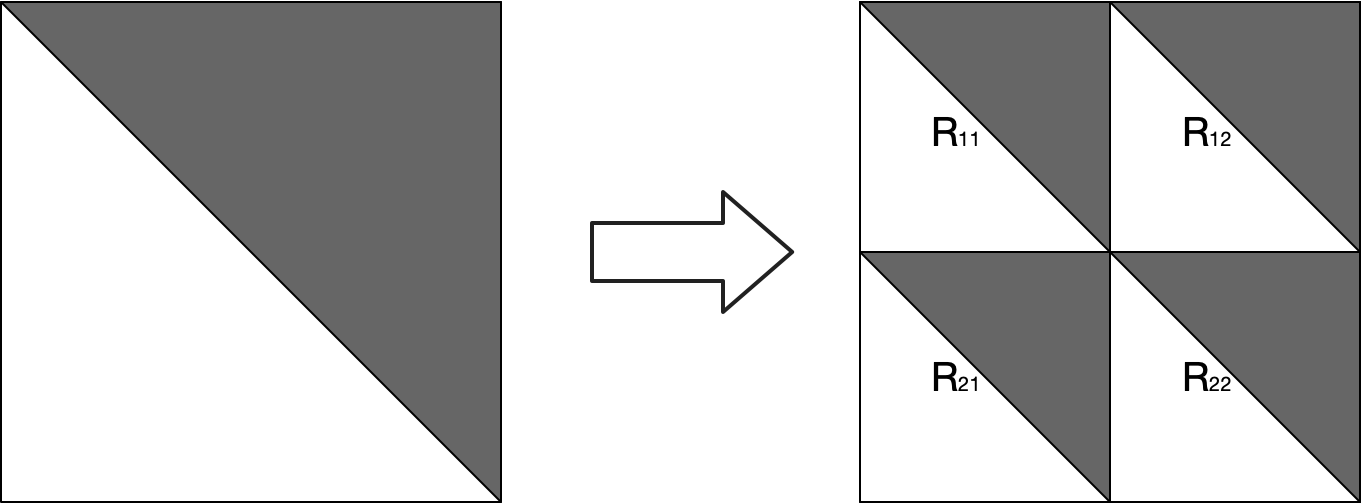
\includegraphics[width=0.45\textwidth,keepaspectratio=true]{Figure_1.png} % Replace with actual file name
        \caption{From $R$ to $R_4$ by permutations }
        \label{fig:Figure_1}
\end{figure}

It is the key to accomplishing the special decomposition \eqref{splitqr}.
\iffalse
{\color{red}V1: Perform swaps on the rows of $R\in \mathbb{R}^{2m \times 2n}$: $r_2\leftrightarrow r_{m +1 + (m \bmod 2)}$, $r_4\leftrightarrow r_{m+3+(m \bmod 2)}$, $\dots$, $r_{m - (m \bmod 2)} \leftrightarrow r_{2m-1}$. Then partition the resulting matrix into  the upper matrix $R_{upper}\in \mathbb{R}^{m \times 2n}$ and the lower matrix $R_{lower}\in \mathbb{R}^{m \times 2n}.$ If $m$ is odd, appending zeros row to the end of the last row of the upper submatrix and prepending zeros row to the beginning of the first row of the lower submatrix ensures that the parity of each row index remains unchanged before the swap, the position of zero rows stays fixed after the swap, and further partitioning is possible. The next is removing the added zeros rows to keep the same size. Subsequently, for the $R_{upper}, R_{lower}$, recursively apply the aforesaid row swapping and partitioning, zero-padding and zero-removing operations to each submatrix until each submatrix contains only two rows; analogous operations are performed on the columns, ultimately yielding the resulting matrix $R_4$.}
\fi 
To better understand the procedure, we will choose the matrix 
\[R= \begin{bmatrix}
 r_{11} & r_{12} & r_{13} & r_{14} & r_{15} & r_{16} & r_{17} & r_{18}\\
 0      & r_{22} & r_{23} & r_{24} & r_{25} & r_{26} & r_{27} & r_{28}\\
 0      & 0      & r_{33} & r_{34} & r_{35} & r_{36} & r_{37} & r_{38}\\
 0      & 0      & 0      & r_{44} & r_{45} & r_{46} & r_{47} & r_{48}\\
 0      & 0      & 0      & 0      & r_{55} & r_{56} & r_{57} & r_{58}\\
 0      & 0      & 0      & 0      & 0      & r_{66} & r_{67} & r_{68}\\
\end{bmatrix}
\]
to \iffalse show how our method works.\fi demonstrate. 

We will first describe how to achieve this in the algorithm, followed by providing the theoretical underpinning for the operation:

We \iffalse perform the following row and column swaps on matrix $R$: \fi
\iffalse 
  Replace the odd rows (1, 3, 5) sequentially with the first three rows. Replace the even rows (2, 4, 6) sequentially with the last three rows. Replace the odd columns (1, 3, 5) sequentially with the first three columns. Replace the even columns (2, 4, 6) sequentially with the last three columns.
  \fi
place the rows (1, 3, 5, 2, 4, 6) of $R$ respectively to the (1, 2, 3, 4, 5, 6) rows of the resulting matrix.  Next, perform column operations on the resulting matrix, place the columns (1, 3, 5, 7, 2, 4, 6, 8) of the resulting matrix respectively to the columns (1, 2, 3, 4, 5, 6, 7, 8). In this way, we can obtain

\iffalse
\[R_4 = \begin{bmatrix}
\begin{array}{cccc:cccc}
 r_{11} & r_{13} & r_{15} & r_{17} & r_{12} & r_{14} & r_{16} & r_{18}\\
 0      & r_{33} & r_{35} & r_{37} & 0      & r_{34} & r_{36} & r_{38}\\
 0      & 0      & r_{55} & r_{57} & 0      & 0      & r_{56} & r_{58}\\
 \cdashline{1-8}
 0      & r_{23} & r_{25} & r_{27} & r_{22} & r_{24} & r_{26} & r_{28}\\
 0      & 0      & r_{45} & r_{47} & 0      & r_{44} & r_{46} & r_{48}\\
 0      & 0      & 0      & r_{67} & 0      & 0      & r_{66} & r_{68}\\
\end{array}
\end{bmatrix}=\begin{bmatrix}
    R_{11} & R_{12}\\R_{21} & R_{22}
\end{bmatrix}.\]
\fi

\begin{align*}
R_4 =
& \begin{bmatrix}
 r_{11} & r_{12} & r_{13} & r_{14} & r_{15} & r_{16} & r_{17} & r_{18}\\
 0      & r_{22} & r_{23} & r_{24} & r_{25} & r_{26} & r_{27} & r_{28}\\
 0      & 0      & r_{33} & r_{34} & r_{35} & r_{36} & r_{37} & r_{38}\\
 0      & 0      & 0      & r_{44} & r_{45} & r_{46} & r_{47} & r_{48}\\
 0      & 0      & 0      & 0      & r_{55} & r_{56} & r_{57} & r_{58}\\
 0      & 0      & 0      & 0      & 0      & r_{66} & r_{67} & r_{68}\\
\end{bmatrix}\\
& \xrightarrow[Step1]{r_{2} \leftrightarrow r_{5}}
\begin{bmatrix}
% \begin{array}{cc:cc:cc}
 r_{11} & r_{12} & r_{13} & r_{14} & r_{15} & r_{16} & r_{17} & r_{18}\\
 0      & 0      & 0      & 0      & r_{55} & r_{56} & r_{57} & r_{58}\\
 0      & 0      & r_{33} & r_{34} & r_{35} & r_{36} & r_{37} & r_{38}\\
 \cdashline{1-8}
 0      & 0      & 0      & r_{44} & r_{45} & r_{46} & r_{47} & r_{48}\\
 0      & r_{22} & r_{23} & r_{24} & r_{25} & r_{26} & r_{27} & r_{28}\\
 0      & 0      & 0      & 0      & 0      & r_{66} & r_{67} & r_{68}\\
% \end{array}
\end{bmatrix}\\
&\xrightarrow[Step2.1]{r_{2} \leftrightarrow r_{3}}
\begin{bmatrix}
% \begin{array}{cc:cc:cc}
 r_{11} & r_{12} & r_{13} & r_{14} & r_{15} & r_{16} & r_{17} & r_{18}\\
 0      & 0      & r_{33} & r_{34} & r_{35} & r_{36} & r_{37} & r_{38}\\
 0      & 0      & 0      & 0      & r_{55} & r_{56} & r_{57} & r_{58}\\
 \cdashline{1-8}
 0      & 0      & 0      & r_{44} & r_{45} & r_{46} & r_{47} & r_{48}\\
 0      & r_{22} & r_{23} & r_{24} & r_{25} & r_{26} & r_{27} & r_{28}\\
 0      & 0      & 0      & 0      & 0      & r_{66} & r_{67} & r_{68}\\
% \end{array}
\end{bmatrix} \\
& \xrightarrow[Step2.2]{r_{4} \leftrightarrow r_{5}}
\begin{bmatrix}
% \begin{array}{cc:cc:cc}
 r_{11} & r_{12} & r_{13} & r_{14} & r_{15} & r_{16} & r_{17} & r_{18}\\
 0      & 0      & r_{33} & r_{34} & r_{35} & r_{36} & r_{37} & r_{38}\\
 0      & 0      & 0      & 0      & r_{55} & r_{56} & r_{57} & r_{58}\\
 0      & r_{22} & r_{23} & r_{24} & r_{25} & r_{26} & r_{27} & r_{28}\\
 0      & 0      & 0      & r_{44} & r_{45} & r_{46} & r_{47} & r_{48}\\
 0      & 0      & 0      & 0      & 0      & r_{66} & r_{67} & r_{68}\\
% \end{array}
\end{bmatrix}\\
& \xrightarrow[Step3.1]{c_{2} \leftrightarrow c_{5}}
\begin{bmatrix}
\begin{array}{cccc:cccc}
 r_{11} & r_{15} & r_{13} & r_{14} &  r_{12} & r_{16} & r_{17} & r_{18}\\
 0      & r_{35} & r_{33} & r_{34} &  0      & r_{36} & r_{37} & r_{38}\\
 0      & r_{55} & 0      & 0      &  0      & r_{56} & r_{57} & r_{58}\\
 0      & r_{25} & r_{23} & r_{24} &  r_{22} & r_{26} & r_{27} & r_{28}\\
 0      & r_{45} & 0      & r_{44} &  0      & r_{46} & r_{47} & r_{48}\\
 0      & 0      & 0      & 0      &  0      & r_{66} & r_{67} & r_{68}\\
\end{array}
\end{bmatrix} \\
& \xrightarrow[Step3.2]{c_{4} \leftrightarrow c_{7}}
\begin{bmatrix}
\begin{array}{cccc:cccc}
 r_{11} & r_{15} & r_{13} & r_{17} & r_{12} & r_{16} & r_{14} & r_{18}\\
 0      & r_{35} & r_{33} & r_{37} & 0      & r_{36} & r_{34} & r_{38}\\
 0      & r_{55} & 0      & r_{57} & 0      & r_{56} & 0      & r_{58}\\
 0      & r_{25} & r_{23} & r_{27} & r_{22} & r_{26} & r_{24} & r_{28}\\
 0      & r_{45} & 0      & r_{47} & 0      & r_{46} & r_{44} & r_{48}\\
 0      & 0      & 0      & r_{67} & 0      & r_{66} & 0      & r_{68}\\
\end{array}
\end{bmatrix}\\
& \xrightarrow[Step4.1]{c_{2} \leftrightarrow c_{3}}
\begin{bmatrix}
\begin{array}{cccc:cccc}
 r_{11} & r_{13} & r_{15} & r_{17} & r_{12} & r_{16} & r_{14} & r_{18}\\
 0      & r_{33} & r_{35} & r_{37} & 0      & r_{36} & r_{34} & r_{38}\\
 0      & 0      & r_{55} & r_{57} & 0      & r_{56} & 0      & r_{58}\\
 0      & r_{23} & r_{25} & r_{27} & r_{22} & r_{26} & r_{24} & r_{28}\\
 0      & 0      & r_{45} & r_{47} & 0      & r_{46} & r_{44} & r_{48}\\
 0      & 0      & 0      & r_{67} & 0      & r_{66} & 0      & r_{68}\\
\end{array}
\end{bmatrix}\\
& \xrightarrow[Step4.2]{c_{6} \leftrightarrow c_{7}}
\begin{bmatrix}
\begin{array}{cccc:cccc}
 r_{11} & r_{13} & r_{15} & r_{17} & r_{12} & r_{14} & r_{16} & r_{18}\\
 0      & r_{33} & r_{35} & r_{37} & 0      & r_{34} & r_{36} & r_{38}\\
 0      & 0      & r_{55} & r_{57} & 0      & 0      & r_{56} & r_{58}\\
 \cdashline{1-8}
 0      & r_{23} & r_{25} & r_{27} & r_{22} & r_{24} & r_{26} & r_{28}\\
 0      & 0      & r_{45} & r_{47} & 0      & r_{44} & r_{46} & r_{48}\\
 0      & 0      & 0      & r_{67} & 0      & 0      & r_{66} & r_{68}\\
\end{array}
\end{bmatrix} \\
&=\begin{bmatrix}
    R_{11} & R_{12}\\R_{21} & R_{22}
\end{bmatrix} = R_4
\end{align*}


\iffalse
\begin{align*}
R
& \xrightarrow{r_{2} \leftrightarrow r_{5}}
\begin{bmatrix}
% \begin{array}{cc:cc:cc}
 r_{11} & r_{12} & r_{13} & r_{14} & r_{15} & r_{16}\\
 0      & 0      & 0      & 0      & r_{55} & r_{56}\\
 0      & 0      & r_{33} & r_{34} & r_{35} & r_{36}\\
 \cdashline{1-6}
 0      & 0      & 0 & r_{44} & r_{45} & r_{46}\\
 0 & r_{22} & r_{23} & r_{24} & r_{25} & r_{26}\\
 0      & 0      & 0      & 0      & 0 & r_{66}\\
% \end{array}
\end{bmatrix}
\xrightarrow{r_{2} \leftrightarrow r_{3}}
\begin{bmatrix}
% \begin{array}{cc:cc:cc}
 r_{11} & r_{12} & r_{13} & r_{14} & r_{15} & r_{16}\\
 0      & 0      & r_{33} & r_{34} & r_{35} & r_{36}\\
 0      & 0      & 0      & 0      & r_{55} & r_{56}\\
 \cdashline{1-6}
 0      & 0      & 0 & r_{44} & r_{45} & r_{46}\\
 0 & r_{22} & r_{23} & r_{24} & r_{25} & r_{26}\\
 0      & 0      & 0      & 0      & 0 & r_{66}\\
% \end{array}
\end{bmatrix} \\
& \xrightarrow{r_{4} \leftrightarrow r_{5}}
\begin{bmatrix}
% \begin{array}{cc:cc:cc}
 r_{11} & r_{12} & r_{13} & r_{14} & r_{15} & r_{16}\\
 0      & 0      & r_{33} & r_{34} & r_{35} & r_{36}\\
 0      & 0      & 0      & 0      & r_{55} & r_{56}\\
 \cdashline{1-6}
 0 & r_{22} & r_{23} & r_{24} & r_{25} & r_{26}\\
 0      & 0      & 0 & r_{44} & r_{45} & r_{46}\\
 0      & 0      & 0      & 0      & 0 & r_{66}\\
% \end{array}
\end{bmatrix}
\xrightarrow{c_{2} \leftrightarrow c_{5}}
\begin{bmatrix}
\begin{array}{ccc:ccc}
 r_{11} & r_{15} & r_{13} & r_{14}  & r_{12} & r_{16}\\
 0      & r_{35} & r_{33} & r_{34}  & 0      & r_{36}\\
 0      & r_{55} & 0      & 0       & 0      & r_{56}\\
 \cdashline{1-6}
 0      & r_{25} & r_{23} & r_{24}  & r_{22} & r_{26}\\
 0      & r_{45} & 0      & r_{44}  & 0      & r_{46}\\
 0      & 0      & 0      & 0       & 0      & r_{66}\\
\end{array}
\end{bmatrix} \\
& \xrightarrow{c_{2} \leftrightarrow c_{3}}
\begin{bmatrix}
\begin{array}{ccc:ccc}
 r_{11} & r_{13} & r_{15} & r_{14}  & r_{12} & r_{16}\\
 0      & r_{33} & r_{35} & r_{34}  & 0      & r_{36}\\
 0      & 0      & r_{55} & 0       & 0      & r_{56}\\
 \cdashline{1-6}
 0      & r_{23} & r_{25} & r_{24}  & r_{22} & r_{26}\\
 0      & 0      & r_{45} & r_{44}  & 0      & r_{46}\\
 0      & 0      & 0      & 0       & 0      & r_{66}\\
\end{array}
\end{bmatrix}
\xrightarrow{c_{4} \leftrightarrow c_{5}}
\begin{bmatrix}
\begin{array}{ccc:ccc}
 r_{11} & r_{13} & r_{15} & r_{12} & r_{14} & r_{16}\\
 0      & r_{33} & r_{35} & 0      & r_{34} & r_{36}\\
 0      & 0      & r_{55} & 0      & 0      & r_{56}\\
 \cdashline{1-6}
0 & r_{23} & r_{25} & r_{22} & r_{24} & r_{26}\\
 0      & 0 & r_{45} & 0      & r_{44} & r_{46}\\
 0      & 0      & 0 & 0      & 0      & r_{66}\\
\end{array}
\end{bmatrix} \\
&=\begin{bmatrix}
    R_{11} & R_{12}\\R_{21} & R_{22}
\end{bmatrix} = R_4
\end{align*}
\fi

\iffalse 
{\color{red}Perform an ordered swap between the even-indexed rows in the upper half and the odd-indexed rows in the lower half of the matrix, then partition it into two upper and lower submatrices (for submatrices with an odd number of rows, appending zeros to the end of the last row of the upper submatrix and prepending zeros to the beginning of the first row of the lower submatrix ensures the parity of each row index remains unchanged before the swap, the position of zero rows stays fixed after the swap, and further partitioning is possible). Subsequently, the above-mentioned row swapping and partitioning operations are recursively applied to each submatrix until each submatrix contains only two rows; analogous operations are performed on the columns, ultimately producing four upper triangular block matrices.}\\
We perform a global row swap \( r_{2} \leftrightarrow r_{5} \), $Step1$, partition the matrix $R$ into upper and lower blocks and swap rows \( r_{2} \leftrightarrow r_{3} \), $Step2.1$, in the upper block and \( r_{4} \leftrightarrow r_{5} \), $Step2.2$, in the lower block, then perform analogue column operations, $Step3-4$. Demonstrate below:
% We can obtain the following resulting matrix:
\begin{align*}
R
& \xrightarrow[Step1]{r_{2} \leftrightarrow r_{5}}
\begin{bmatrix}
% \begin{array}{cc:cc:cc}
 r_{11} & r_{12} & r_{13} & r_{14} & r_{15} & r_{16}\\
 0      & 0      & 0      & 0      & r_{55} & r_{56}\\
 0      & 0      & r_{33} & r_{34} & r_{35} & r_{36}\\
 \cdashline{1-6}
 0      & 0      & 0 & r_{44} & r_{45} & r_{46}\\
 0 & r_{22} & r_{23} & r_{24} & r_{25} & r_{26}\\
 0      & 0      & 0      & 0      & 0 & r_{66}\\
% \end{array}
\end{bmatrix}
\xrightarrow[Step2.1]{r_{2} \leftrightarrow r_{3}}
\begin{bmatrix}
% \begin{array}{cc:cc:cc}
 r_{11} & r_{12} & r_{13} & r_{14} & r_{15} & r_{16}\\
 0      & 0      & r_{33} & r_{34} & r_{35} & r_{36}\\
 0      & 0      & 0      & 0      & r_{55} & r_{56}\\
 \cdashline{1-6}
 0      & 0      & 0 & r_{44} & r_{45} & r_{46}\\
 0 & r_{22} & r_{23} & r_{24} & r_{25} & r_{26}\\
 0      & 0      & 0      & 0      & 0 & r_{66}\\
% \end{array}
\end{bmatrix} \\
& \xrightarrow[Step2.2]{r_{4} \leftrightarrow r_{5}}
\begin{bmatrix}
% \begin{array}{cc:cc:cc}
 r_{11} & r_{12} & r_{13} & r_{14} & r_{15} & r_{16}\\
 0      & 0      & r_{33} & r_{34} & r_{35} & r_{36}\\
 0      & 0      & 0      & 0      & r_{55} & r_{56}\\
 % \cdashline{1-6}
 0 & r_{22} & r_{23} & r_{24} & r_{25} & r_{26}\\
 0      & 0      & 0 & r_{44} & r_{45} & r_{46}\\
 0      & 0      & 0      & 0      & 0 & r_{66}\\
% \end{array}
\end{bmatrix}
\xrightarrow[Step3]{c_{2} \leftrightarrow c_{5}}
\begin{bmatrix}
\begin{array}{ccc:ccc}
 r_{11} & r_{15} & r_{13} & r_{14}  & r_{12} & r_{16}\\
 0      & r_{35} & r_{33} & r_{34}  & 0      & r_{36}\\
 0      & r_{55} & 0      & 0       & 0      & r_{56}\\
 0      & r_{25} & r_{23} & r_{24}  & r_{22} & r_{26}\\
 0      & r_{45} & 0      & r_{44}  & 0      & r_{46}\\
 0      & 0      & 0      & 0       & 0      & r_{66}\\
\end{array}
\end{bmatrix} \\
& \xrightarrow[Step4.1]{c_{2} \leftrightarrow c_{3}}
\begin{bmatrix}
\begin{array}{ccc:ccc}
 r_{11} & r_{13} & r_{15} & r_{14}  & r_{12} & r_{16}\\
 0      & r_{33} & r_{35} & r_{34}  & 0      & r_{36}\\
 0      & 0      & r_{55} & 0       & 0      & r_{56}\\
 % \cdashline{1-6}
 0      & r_{23} & r_{25} & r_{24}  & r_{22} & r_{26}\\
 0      & 0      & r_{45} & r_{44}  & 0      & r_{46}\\
 0      & 0      & 0      & 0       & 0      & r_{66}\\
\end{array}
\end{bmatrix}
\xrightarrow[Step4.2]{c_{4} \leftrightarrow c_{5}}
\begin{bmatrix}
\begin{array}{ccc:ccc}
 r_{11} & r_{13} & r_{15} & r_{12} & r_{14} & r_{16}\\
 0      & r_{33} & r_{35} & 0      & r_{34} & r_{36}\\
 0      & 0      & r_{55} & 0      & 0      & r_{56}\\
 \cdashline{1-6}
0 & r_{23} & r_{25} & r_{22} & r_{24} & r_{26}\\
 0      & 0 & r_{45} & 0      & r_{44} & r_{46}\\
 0      & 0      & 0 & 0      & 0      & r_{66}\\
\end{array}
\end{bmatrix} 
% &=\begin{bmatrix}
%     R_{11} & R_{12}\\R_{21} & R_{22}
% \end{bmatrix}
= R_4
\end{align*}
 \fi
 \iffalse 
The above process applies to any upper triangular matrices $R$ with even orders $2m \times 2n$. Below, we will explain why aforesaid  operations are performed.
\fi
By the properties of the row and column transformations, we can check that the relationship between $R$ and $R_4$ is as follows:
\begin{equation}\label{eq:Rn}
    P_{m} R P_{n}^T = \begin{bmatrix} R_{11} & R_{12}\\R_{21}& R_{22}\end{bmatrix}.
\end{equation}
To obtain the matrix $P_k, k\in \{m,n\}$ for $R \in \mathbb{R}^{2m \times 2n}$, we established Algorithm \ref{alg:Permutation} when the input is $P=I_{2k}$, and obtain the permutation matrix $P_k$:

\begin{equation}\label{p}
    P_k = \begin{bmatrix} 
            1 & 0 & 0 & 0 & \cdots & 0 & 0\\ 
            0 & 0 & 1 & 0 & \cdots & 0 & 0\\ 
            \vdots & \vdots & \vdots & \vdots &  & \vdots & \vdots\\ 
            0 & 0 & 0 & 0 & \cdots & 1 & 0 \\
            0 & 1 & 0 & 0 & \cdots & 0 & 0\\ 
            0 & 0 & 0 & 1 & \cdots & 0 & 0\\ 
            \vdots & \vdots & \vdots & \vdots &  & \vdots & \vdots\\ 
            0 & 0 & 0 & 0 &\cdots & 0 & 1 
        \end{bmatrix}_{2k \times 2k}.
\end{equation}

This $P_k$ and \eqref{eq:Rn} explain why we perform aforesaid operations on $R$.

After completing the above steps, we can now proceed to implement the decomposition \eqref{splitqr}.
First, perform the QR decomposition:
\[P_m^TA^\sigma P_n = \widehat{Q}\widehat{R}.\]
According to \eqref{eq:Rn}, we have
\[P_m^TA^\sigma P_n = \widehat{Q}\widehat{R} = \widehat{Q}(P_m^TR_4P_n).\]
Multiplying both sides of the equation by $P_m$ on the left and $P_n^T$ on the right yields
\[A^\sigma=P_m\widehat{Q}P_m^T R_4.\]
 Since $P_m$ is a permutation matrix, it is also an orthogonal matrix. Thus, the product of matrices, $P_m\widehat{Q}P_m^T$, is also an orthogonal matrix. Then we get our required special decomposition \[A^\sigma=\widetilde{Q}R_4,\] where $\widetilde{Q}=P_m\widehat{Q}P_m^T$ is orthogonal, and $R_4$ is in the form of \eqref{r4}. During the process, we need to compute 
$P_m^TA^\sigma P_n, P_m\widehat{Q}P_m^T, P_m \widehat{R}P_n^T$. To reduce computational cost, we designed Algorithm \ref{alg:Permutation Optimization} to avoid multiplication operations on $A^\sigma, \widehat{Q}, \widehat{R}$.
\iffalse
{\color{red}To reduce computational cost, we designed Algorithm \ref{alg:Permutation Optimization}, which avoids multiplication operations on $A^\sigma, \widehat{R}, \widehat{Q}$.}\fi

\end{multicols}
\begin{algorithm}[htbp]
    \caption{Matrix Permutation Recursive Algorithm} \label{alg:Permutation}
    \begin{algorithmic}[1]
    \Function{Permutation}{$P$}
        \State \% \textbf{Input:} $P \in \mathbb{R}^{2s \times 2n}$, the matrix to permuting.
        \State \% \textbf{Output:} $P \in \mathbb{R}^{2s \times 2n}$, the matrix after permuted.
        % \State \% \textbf{Step 1} Recursive stop condition:
        \If{$s=1$} \qquad\qquad\qquad\qquad\qquad\qquad\qquad\qquad \ \% \textbf{Step 1} Recursive stop when $s=1$.
            \State \Return \ $P$;
        \End 
        % \State \% \textbf{Step 2} Initialization:
        \State $s2 = \text{floor}(s/2)$;\qquad\qquad\qquad\qquad\qquad\qquad\quad \ \% \textbf{Step 2} Initialize $s2$.
        \For{$i=1:s2$} \qquad\qquad\qquad\qquad\qquad\qquad\qquad\% \textbf{Step 3} Swap even rows in the upper half of $P$ with
            \If{$\text{mod}(s, 2)=0$} \qquad\qquad\qquad\qquad\qquad\quad \ \% \qquad\quad\ \  odd rows in the lower half of $P$.
                \State $P= \text{swap}(P,2*i,s+2*i-1)$;
            \Else
                \State $P= \text{swap}(P,2*i,s+2*i)$;
            \End
            % \State $P= \text{swap}(P,2*i,s+2*i-1+\text{mod}(s, 2))$;
        \End
        \If{$\text{mod}(s, 2)=1$} \qquad\qquad\qquad\qquad\qquad\qquad\ \% \textbf{Step 4} Partition matrix. Add zero rows, if $s$ is odd.
            \State $P_{upper} = [P(1:s,:); \text{zeros}(1, 2n)]$;
            \State $P_{lower} = [\text{zeros}(1, 2n); P(s+1:end)]$;
            % \If{flag=1} \qquad\qquad\qquad\qquad\qquad\qquad\qquad\qquad\qquad\ \ \% \qquad\quad\ \ ensure submatrix has even rows.
            % \Else
            %     \State $P_{lower} = [P; \text{zeros}(1, \text{size}(P, 2))]$;
            % \End
        \Else
            \State $P_{upper} = P(1:s,:)$;
            \State $P_{lower} = P(s+1:end)$;
        \End
        % \State $P_{upper} = \text{mod}(s, 2)=1 ? [P(1:s,:); \text{zeros}(1, 2n)] : P(1:s,:)$;
        % \State $P_{lower} = \text{mod}(s, 2)=1 ? [\text{zeros}(1, 2n) ; P(s+1:end)] : P(s+1:end)$;
        
        \State $P_{upper} = \text{Permutation}(P_{upper})$; \qquad\qquad\qquad\% \textbf{Step 5} Recursive executing.
        \State $P_{lower} = \text{Permutation}(P_{lower})$;
        \If{$\text{mod}(s, 2)=1$} \qquad\qquad\qquad\qquad\qquad\qquad\ \% \textbf{Step 6} Remove zero rows, if $s$ is odd.
            \State $P(1:s) = P_{upper}(1:s, :)$;
            \State $P(s+1:end) = P_{lower}(2:end, :)$;
        \Else
            \State $P(1:s) = P_{upper}(1:end, :)$;
            \State $P(s+1:end) = P_{lower}(1:end, :)$;
        \End
        % \State $P(1:s) = P_{upper}(1:end-text{mod}(s, 2), :)$;
        % \State $P(s+1:end) = P_{lower}(1+text{mod}(s, 2):end, :)$;
    \End 
    \end{algorithmic}
\end{algorithm}
% \begin{multicols}{2}
% \end{multicols}
\begin{algorithm}[htbp]
    \caption{Matrix Permutation Optimization Algorithm}
    \label{alg:Permutation Optimization}
    \begin{algorithmic}[1]
    \Function{PermutationOpt}{$A,t$}
        \State \% \textbf{Input:} $ A\in \mathbb{R}^{2m\times 2n}$, $t$ is 0 or 1.
        \State \% \textbf{Output:} $B \in\mathbb{R}^{2m\times 2n}$, such that $B=P_mA$ when $t$ is $0$;  $B=P_m^TA$ when $t$ is $1$.
        \If {$t == 0$}
          \For {$i = 1:m$} \qquad\qquad\qquad\qquad \% 
          %Copy odd rows of A to B's 1–m and even rows to B's m+1–2m.
          % Odd rows of A → B[1:m], even rows → B[m+1:2m]
          Assign odd rows of $A$ sequentially to the $1$st-$m$th rows of $B$; 
            \State $B(i, :) = A(2*i-1, :);$
            \qquad\ \% even rows of $A$ sequentially to the $(m+1)$th-$2m$th rows of $B$.
            \State $B(m+i, :) = A(2*i, :);$
          \End
        \Else  
            \For {$i = 1:m$} \qquad\qquad\qquad\qquad \% 
            Assign $A$'s $1$th--$m$th rows sequentially to odd rows of $B$;
            % A[1:m] → odd rows of B, A[m+1:2m] → even rows of B
            \State $B(2*i-1, :) = A(i, :);$ \qquad\ \%  $A$'s $(m+1)$th--$2m$th rows sequentially to even rows of $B$.
            \State $B(2*i, :) = A(m+i, :);$
          \End
        \End
    \End 
    \end{algorithmic}
\end{algorithm}

\begin{multicols}{2}
\textbf{Step 2:} Using equation \eqref{eq:2.3}, construct the matrix $R$ such that $R^\sigma=R_4:$
\begin{equation*}
R = \frac{R_{11} + R_{22}}{2} + \frac{R_{21} - R_{12}}{2}i + \frac{R_{11} - R_{22}}{2}j + \frac{R_{21} + R_{12}}{2}k,
\end{equation*}
Since $R_{11}, R_{12}, R_{21}, R_{22}$ are upper triangular, this ensures that the constructed split quaternion matrix $R$ is also upper triangular. Additionally, construct the matrix $Q$ such that $Q^\sigma=\widetilde{Q}:$
\begin{equation*}
Q = \frac{Q_{11} + Q_{22}}{2} + \frac{Q_{21} - Q_{12}}{2}i + \frac{Q_{11} - Q_{22}}{2}j + \frac{Q_{21} + Q_{12}}{2}k,
\end{equation*}
where $Q_{11}, Q_{12}, Q_{21}, Q_{22} \in \mathbb{R}^{m \times n}$ are the blocks of the orthogonal matrix $\widetilde{Q} = \begin{bmatrix} Q_{11} & Q_{12} \\ Q_{21} & Q_{22} \end{bmatrix} \in \mathbb{R}^{2m \times 2m}$. Note that \[(Q^H Q)^\sigma = {(Q^H)}^\sigma Q^\sigma = {(Q^\sigma)}^TQ^\sigma = \widetilde{Q}^T\widetilde{Q} = I_{2m},\] indicating that the split quaternion matrix $Q$ remains a unitary matrix.

Now, $A^\sigma=\widetilde{Q}R_4=Q^\sigma R^\sigma$ implies
$A = Q R$, as required.

From the process described above, any split quaternion matrix can be decomposed into QR decomposition. Our results can be summarized as follows:
\begin{theorem}(QR Decomposition)
    Let $A \in \mathbb{H}_s^{m \times n}$. There exist a unitary matrix $Q \in \mathbb{H}_s^{m \times m}$ and an upper triangular matrix $R \in \mathbb{H}_s^{m \times n}$ such that
    \begin{eqnarray}\label{eq:split QR}
        A = Q R.
    \end{eqnarray}
\end{theorem}
% \iffalse
% To reduce the computational cost, we designed Algorithm \ref{alg:Permutation Optimization}, which avoids multiplication operations on $\widehat{A}, \widehat{R}, \widehat{Q}$.

\textbf{Complexity Analysis:}
{Complexity Analysis:} For a split quaternion matrix $A = A_0 + A_1i + A_2j + A_3k \in \mathbb{H}_s^{m \times n}$, the computational complexity of Algorithm \ref{alg:QR} is dominated by three components:  

\textbf{1. Real Representation Conversion:}
Constructing the real representation $A^\sigma \in \mathbb{R}^{2m \times 2n}$ requires about $4mn$ flops. 

\textbf{2. Permutations On $A^\sigma, \widehat{Q}, \widehat{R}$:}
By using Algorithm \ref{alg:Permutation Optimization},  which requires approximately  $(8m+4n)$ flops.

\textbf{3. Real Matrix QR Decomposition:}
The QR decomposition of $A^\sigma \in \mathbb{R}^{2m \times 2n}$ using Householder reflections dominates the complexity at $16(mn^2-\frac{n^3}{3})$ flops.

\textbf{Total Complexity}
$$
\underbrace{(4mn)}_{\text{Real Rep.}} + \underbrace{(8m+4n)}_{\substack{\text{Permutation} \\ \text{(optimized)}}} + \underbrace{(16(mn^2-\frac{n^3}{3}))}_{\text{QR}} \approx \boxed{(16(mn^2-\frac{n^3}{3}))}
$$  
% \fi

\end{multicols}
\begin{algorithm}[htbp] 
    \caption{Compute the QR of Split Quaternion Matrix \(A\)}
    \label{alg:QR}
    \begin{algorithmic}[1]
    \Function{Split-QR}{$A$}
        \State \% \textbf{Input:} \(A = A_0 + A_1 i + A_2 j + A_3 k \in \mathbb{H}_s^{m\times n}\).
        \State \% \textbf{Output:} Unitary matrix \(Q \in \mathbb{H}_s^{m\times m}\), upper triangular matrix \(R \in \mathbb{H}_s^{m\times n}\), satisfying \(Q  R = A\).
        % \State \% \textbf{Step 1} Real representation of $A$:
        \State \(A^\sigma = \begin{bmatrix}
            A_0 + A_2 & -A_1 + A_3 \\ 
            A_1 + A_3 & A_0 - A_2
            \end{bmatrix} \in \mathbb{R}^{2m\times 2n}\); \qquad\qquad\qquad\qquad \% \textbf{Step 1} Real representation of $A$.
        
        % \State \% \textbf{Step 2} Compute \(\widehat{A} = P_{m}^T A^\sigma P_{n}\): 
        \State $\widehat{A}=\text{PermutationOpt}(A^\sigma,1);$  \qquad\qquad\qquad\qquad\qquad\qquad\quad\% \textbf{Step 2} Compute \(\widehat{A} = P_{m}^T A^\sigma P_{n}\).
        \State $\widehat{A}=\text{PermutationOpt}(\widehat{A}',1),\widehat{A}=\widehat{A}';$
        
        % \State \% \textbf{Step 3} Compute QR:
        \State \([\widehat{Q},\widehat{R}] = \text{qr}(\widehat{A})\); \qquad\qquad\qquad\qquad\qquad\qquad\qquad\qquad\qquad\quad\% \textbf{Step 3} Compute QR of $\widehat{A}$.
        
        % \State \% \textbf{Step 4} Compute \(R^\sigma = P_{m}\widehat{R}P_{n}^T\), \(Q^\sigma =      P_{m}\widehat{Q}P_{m}^T\): 
        \State $\widehat{R}=\text{PermutationOpt}(\widehat{R},0)$; \qquad\qquad\qquad\qquad\qquad\qquad\quad\ \ \% \textbf{Step 4} Compute \(R^\sigma = P_{m}\widehat{R}P_{n}^T\), 
        \State $\widehat{R}=\text{PermutationOpt}(\widehat{R}',0);R^\sigma=\widehat{R}'$;\qquad\qquad\qquad\qquad\quad\ \ \% \qquad\quad \ \(Q^\sigma = P_{m}\widehat{Q}P_{m}^T\).
        \State $\widehat{Q}=\text{PermutationOpt}(\widehat{Q},0)$;
        \State $\widehat{Q}=\text{PermutationOpt}(\widehat{Q}',0);Q^\sigma=\widehat{Q}'$;
        
        % \State \% \textbf{Step 5} Construct matrix Q, R:
        \State $Q_0 = (Q^\sigma(1\!:\!m,1\!:\!m) + Q^\sigma(m+1\!:\!2m,m+1\!:\!2m))/2$; \qquad\ \% \textbf{Step 5} Construct matrix Q, R.
        \State $Q_1 = (Q^\sigma(m+1\!:\!2m,1\!:\!m) - Q^\sigma(1\!:\!m,m+1\!:\!2m))/2$;
        \State $Q_2 = (Q^\sigma(1\!:\!m,1\!:\!m) - Q^\sigma(m+1\!:\!2m,m+1\!:\!2m))/2$;
        \State $Q_3 = (Q^\sigma(m+1\!:\!2m,1\!:\!m) + Q^\sigma(1\!:\!m,m+1\!:\!2m))/2$;
        \State $R_0 = (R^\sigma(1\!:\!m,1\!:\!n) + R^\sigma(m+1\!:\!2m,n+1\!:\!2n))/2$;
        \State $R_1 = (R^\sigma(m+1\!:\!2m,1\!:\!n) - R^\sigma(1\!:\!m,n+1\!:\!2n))/2$;
        \State $R_2 = (R^\sigma(1\!:\!m,1\!:\!n) - R^\sigma(m+1\!:\!2m,n+1\!:\!2n))/2$;
        \State $R_3 = (R^\sigma(m+1\!:\!2m,1\!:\!n) + R^\sigma(1\!:\!m,n+1\!:\!2n))/2$;

        % \State \% \textbf{Step 6} Return: 
        \State $Q = Q_0 + Q_1i + Q_2j + Q_3k$; \qquad\qquad\qquad\qquad\qquad\qquad\qquad\% \textbf{Step 6} Return $Q, R$.
        \State $R = R_0 + R_1i + R_2j + R_3k$;
    \End 
    \end{algorithmic}
\end{algorithm}
\begin{multicols}{2}


\section{Numerical Examples}
\iffalse In this section,  we will use the proposed Algorithm 2 to compute the QR decomposition for split quaternion matrices and apply it to solving a matrix equation.\fi
In this section, we will use the proposed Algorithm \ref{alg:QR} to compute the QR decomposition for split quaternion matrices.
\begin{example}
    Given a split quaternion matrix $A = A_{0}+A_{1}i+A_{2}j+A_{3}k\in \mathbb{H}_s^{m\times n}$, where
    \begin{equation}
       \begin{cases}
            m = 50,100,\cdots,1000;\\
            n = 50,100,\cdots,1000;  \\
            A_{0}=\text{rand}(m,n);
            A_{1}=\text{rand}(m,n); \\
            A_{2}=\text{rand}(m,n);
            A_{3}=\text{rand}(m,n).
        \end{cases} \label{eq:example2}
    \end{equation}
\end{example}
Here, the MATLAB function $rand(m,n)$ is used to generate a $m \times n$ real matrix with random elements that fall within the interval (0,1).  All experiments were performed and computed using MATLAB 2024a on a system equipped with an 11th Gen Intel(R) Core(TM) i7-1185G7 @ 3.00GHz processor, 16.0 GB RAM and Windows 11 Pro. We executed Algorithm \ref{alg:QR} to perform the QR decomposition on $A$, and have calculated the CPU time and the relative error
$\epsilon = \frac{\left\|A - Q R\right\|_{F}}{\|A\|_{F}}.$
The experimental results from Figure \ref{fig:Figure_2} show that Algorithm \ref{alg:QR} performs quite well in both speed and accuracy. 
\begin{figure}[H]
    \centering
    \begin{minipage}[b]{0.45\textwidth}
        \centering
        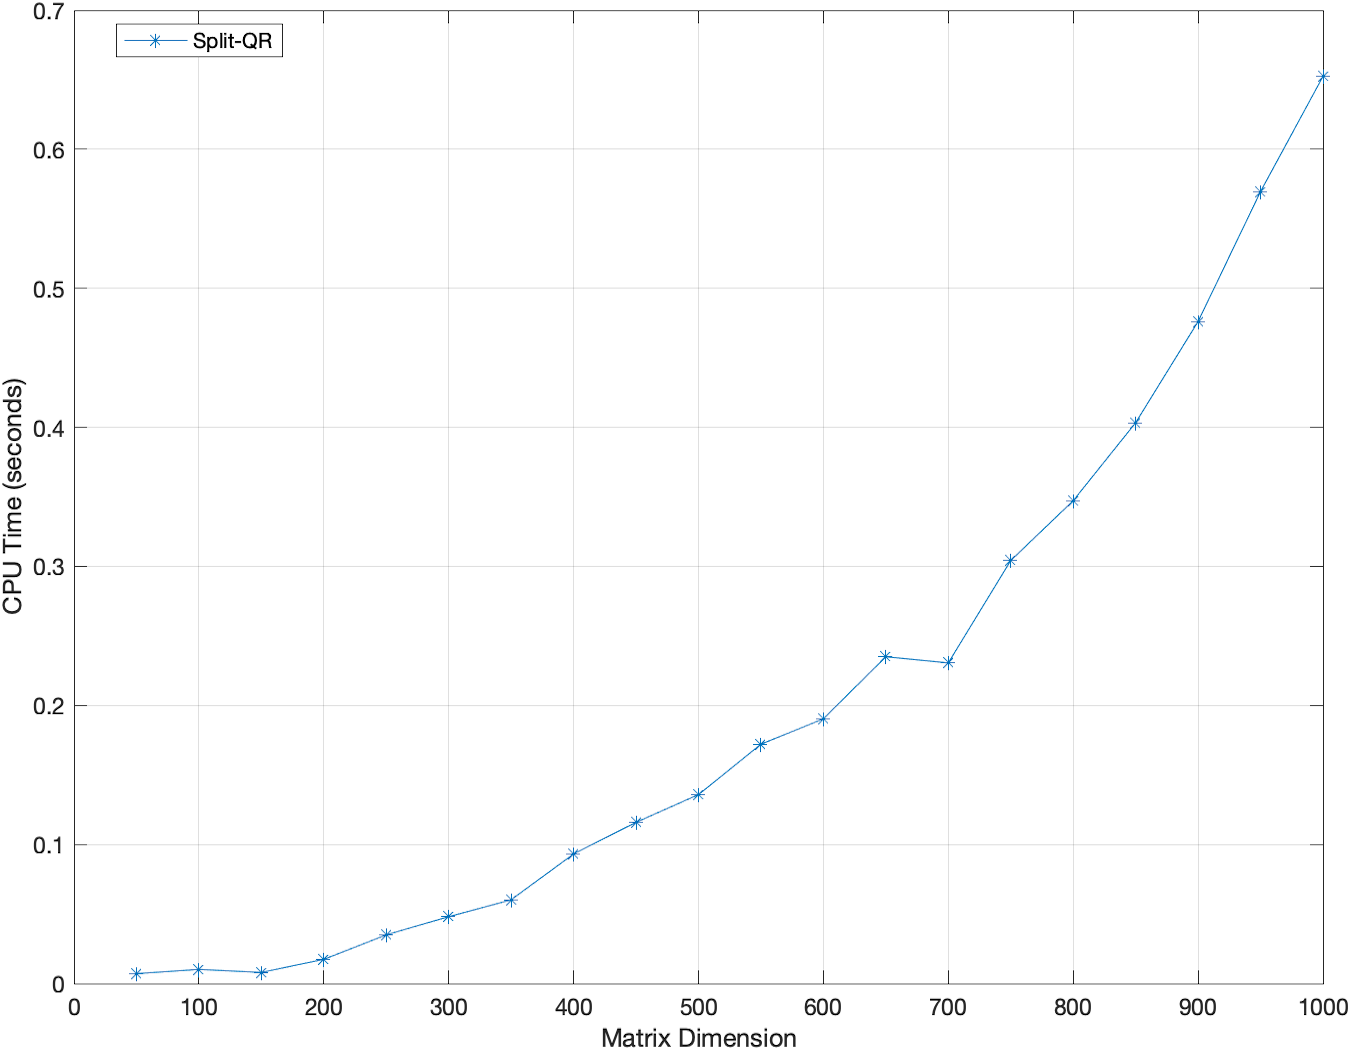
\includegraphics[width=\textwidth]{Figure_2.png} % Replace with actual filename
       % \subcaption{(a)}
    \end{minipage}
    \hfill % Add space
    \begin{minipage}[b]{0.45\textwidth}
        \centering
        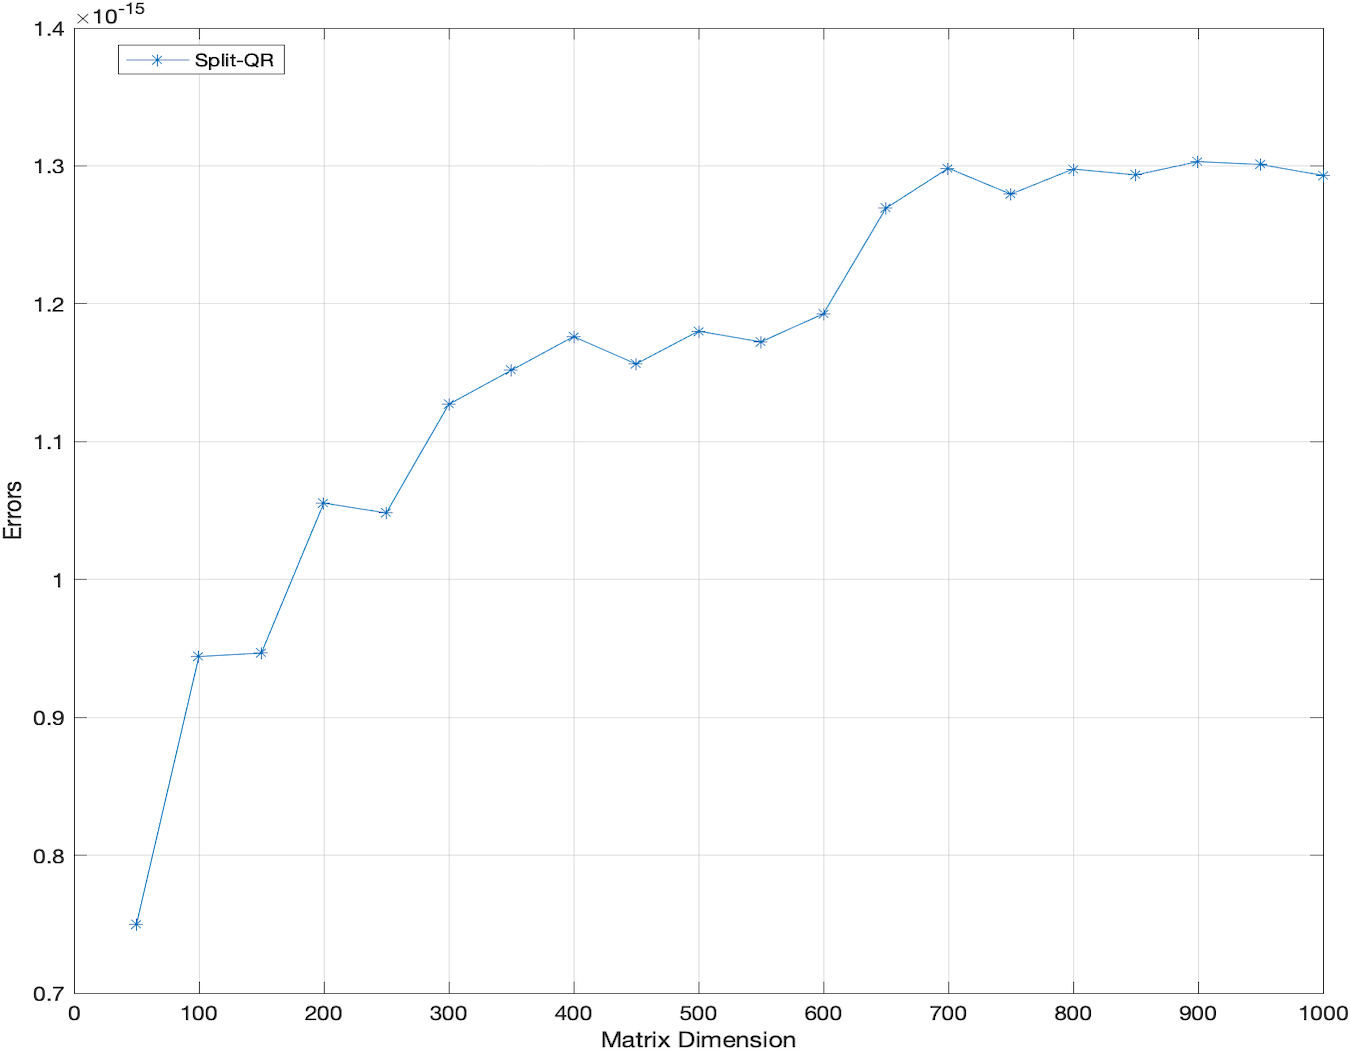
\includegraphics[width=\textwidth]{Figure_3.png} % Replace with actual filename
        % \subcaption{(b)}
    \end{minipage}
    % \captionsetup{font=footnotesize}
    \caption{ CPU Time and Error Analysis of the QR Algorithm for Split Quaternion Matrices }
     \label{fig:Figure_2}
\end{figure}

In the following, we will discuss the application of QR decomposition in solving matrix equations.
\begin{example}
Utilize the QR algorithm to solve the split quaternion matrix equation $AX = B$, where
\begin{align*}
  A &=
    \begin{bmatrix}
    -4 & -2 & -8 \\
    -2 & -2 & -5 \\
     7 & -3 & -9
    \end{bmatrix} +
    \begin{bmatrix}
    -1 & -2 &  4 \\
    -5 & -8 & -5 \\
    -4 &  0 &  6
    \end{bmatrix} i \\
    &+ 
    \begin{bmatrix}
    -9  & -6  & -8 \\
    -2  & -10 & -5 \\
    -10 & -7  & -7
    \end{bmatrix} j +
    \begin{bmatrix}
    -8 &  9 & -3 \\
     2 & -6 &  0 \\
     8 &  0 & -5
    \end{bmatrix} k,
\end{align*}
\begin{align*}
  B &=
    \begin{bmatrix}
    -9 & -10 &  10 \\
    -1 &  10 &  6 \\
    -7 & -1  & -10
    \end{bmatrix} +
    \begin{bmatrix}
    4 &  1 & -6 \\
    4 & -6 & -3 \\
    3 &  6 &  8
    \end{bmatrix} i \\
    &+
    \begin{bmatrix}
     7 & 2 &  2 \\
    -2 & 9 & -4 \\
    -4 & 9 &  7
    \end{bmatrix} j +
    \begin{bmatrix}
    -1 &   1 & -3 \\
     8 &   5 & -7 \\
    -10 & -7 & -4
    \end{bmatrix} k.
\end{align*}
\end{example}  

First, using Algorithm \ref{alg:QR} to perform QR decomposition on $A$ to obtain $Q$ and $R:$
\setlength{\jot}{2pt}
\setlength{\arraycolsep}{1pt}
% {\footnotesize
\begin{align*}
  Q &=
     \begin{bmatrix}
    -0.514 & -0.047 & -0.344 \\
    -0.126 & -0.411 & -0.041 \\
    -0.436 & -0.429 & -0.099
    \end{bmatrix} +
    \begin{bmatrix}
    -0.363 &  0.479 &  0.122 \\
     0.077 & -0.458 & -0.100 \\
     0.383 & -0.194 &  0.138
    \end{bmatrix} i \\
    & + 
    \begin{bmatrix}
    -0.236 & -0.062 & -0.155 \\
    -0.105 &  0.031 &  0.403 \\
     0.262 &  0.178 & -0.296
    \end{bmatrix} j +
    \begin{bmatrix}
    -0.157 &  0.171 &  0.319 \\
    -0.250 & -0.133 &  0.577 \\
    -0.152 &  0.291 & -0.343
    \end{bmatrix} k,
\end{align*}
\begin{align*}
  R &=
     \begin{bmatrix}
    -3.041 & 3.419 & 10.927 \\
     0     & 6.061 & 6.456 \\
     0     & 0     & 7.714
    \end{bmatrix} +
    \begin{bmatrix}
    -1.443 & 8.617 &  1.053 \\
     0     & 1.847 & -2.947 \\
     0     & 0     & -5.025
    \end{bmatrix} i \\
    &+ 
    \begin{bmatrix}
    20.361 & 5.876  & 6.740 \\
     0     & 14.697 & 6.795 \\
     0     & 0      & 0.815
    \end{bmatrix} j +
    \begin{bmatrix}
    1.443 & -2.642 &  6.596 \\
    0     & -1.847 & -1.528 \\
    0     &  0     &  5.025
    \end{bmatrix} k.
\end{align*}
% }
Thus, the equation can be rewritten as
\begin{equation}
    QRX = B.\label{eq:example1}
\end{equation}

Since $Q$ is a unitary matrix, multiplying both sides of \eqref{eq:example1} by $Q^H$ from the left yields $RX = Q^HB\triangleq \widehat{B}$,
where
% {\footnotesize
\begin{align*}
  \widehat{B} &=
    \begin{bmatrix}
     4.981  &  6.383  &  8.076 \\
    -2.019  & -1.922  & -1.440 \\
     11.356 &  10.929 & -9.652
    \end{bmatrix} +
    \begin{bmatrix}
    -1.144 & -7.725  &  6.206 \\
     1.152 &  11.947 & -2.239 \\
    -3.761 &  0.482  & -0.749
    \end{bmatrix} i \\ &+
    \begin{bmatrix}
    -6.136 & -7.249 & -9.693 \\
     0.310 & -4.646 &  0.574 \\
     1.391 & -2.620 & -3.994
    \end{bmatrix} j +
    \begin{bmatrix}
     11.385 & -4.261 & -2.859 \\
    -7.851  &  1.655 & -0.404 \\
    -0.653  &  6.826 &  12.841
    \end{bmatrix} k.
\end{align*}
% }
Note that $R$ is an upper triangular matrix. Thus, $RX = Q^HB\triangleq \widehat{B}$ can be solved using back substitution:
% {\footnotesize
 \begin{align*}
  X &=
    \begin{bmatrix}
    -1.082 & -0.797 &  1.407 \\
    -0.316 & -0.028 &  0.749 \\
     1.846 &  0.845 & -2.243
    \end{bmatrix} +
    \begin{bmatrix}
    -1.116 & -0.337 &  0.999 \\
    -0.423 & -0.961 &  1.907 \\
     0.349 &  1.315 & -0.403
    \end{bmatrix} i \\ &+
    \begin{bmatrix}
    -0.456 & -0.123 &  1.793 \\
    -1.222 & -0.449 &  1.810 \\
     0.402 & -1.119 & -1.423
    \end{bmatrix} j +
    \begin{bmatrix}
     0.944 &  0.982 & -1.597 \\
     0.059 & -0.514 &  0.229 \\
    -0.989 & -0.256 &  2.156
    \end{bmatrix} k.
\end{align*}
% }
And the relative error is $\frac{\|AX - B\|_F}{\|B\|_F} = 1.2412\times 10^{-15}$.

\section{Acknowledgments}
This research is supported by \iffalse Macao Science and Technology Development Fund (No. 0013/2021/ITP),\fi the grants from \iffalse  the National Natural Science Foundation of China (12371023, 12271338),\fi NSF of China (12371023, 12271338) and \iffalse the Natural Sciences and Engineering Research Council of Canada (NSERC) (RGPIN 2020-06746).\fi Canada NSERC.

{\bf Data availability:} No data was used for the research described in the article.

%-------------------- 参考文献 --------------------
\parskip=5pt
\noindent \rule[0pt]{25em}{1pt}

\parskip=10pt

\renewcommand{\bibname}{}

\noindent {\References{References}}
\vspace{-60pt}
% \begin{list}{[\arabic{enumi}]}{\usecounter{enumi} %%
% \leftmargin=2em%%%%%%
% \labelsep=1em%%%%%
% \renewcommand{\makelabel}[1]{#1 \hfil}}%%

% natbib的用法
\bibliographystyle{elsarticle-num} % 参考文献样式
\let\clearpage\relax
\bibliography{references} % 文献数据库文件名

% biblatex的用法
% \printbibliography


\end{multicols}
\end{document}